
\documentclass[aps,twocolumn,secnumarabic,nobalancelastpage,amsmath,amssymb,
nofootinbib]{revtex4}

% nofootinbib is another document class option that allows you to put
% footnotes on the page where they occur rather than at the end of the
% paper.  This makes for easier reading!

% secnumarabic is a particularly nice way of identifying sections by
% number to aid electronic review and commentary.

% amsmath and amssymb are necessary for the subequations environment
% among others

\usepackage{chapterbib}
\usepackage{color}
\usepackage{graphics}      % standard graphics specifications
\usepackage{graphicx}      % alternative graphics specifications
\usepackage{longtable}     % helps with long table options
%\usepackage{url}          % for on-line citations (conflicts with hyperref)
\usepackage{bm}            % special 'bold-math' package
\usepackage[colorlinks=true]{hyperref}


\begin{document}
\title{Poisson Statistics}
\author         {Adnan Basar (Partner: Kadir Simsek)}
\email          {adnanbasarr@icloud.com}
\affiliation    {2010205108}
\date{\today}





\begin{abstract}
In this experiment, poisson statistics are going to be examined by using randomness property of radioactive decay. 
\end{abstract}

\maketitle

%%%%%%%%%%%%%%%%%%%%%%%%%%%%%%%%%%%%%%%%%%%%%%%%%%%%%%%%%%%%%%%%%%
\section{Introduction}
Radioactive decay is a random process in which the emission of radiation depends on the 
number of atoms that can decay and a probability function that is characteristic their 
natural lifetimes. The detection of particles is random and any two measurements of the 
particles over equal periods of time will most likely be different. For large numbers, the 
difference between the measurements will be a small percentage. The probability of 
detecting a specific number of events for a given measurement is given by the standard 
normal or Gaussian distribution as was studied in the experiment on statistical analysis. 
However, for the measurement of a small number of events, the probability distribution 
for detecting a specific number of events is different and is given by a Poisson 
distribution.\\

For rare events, the average number detected might also be much less than one, The 
Poisson distribution applies to these measurements and is useful for determining the 
probability of detecting a single event or more than one event in the same period. The 
Poisson distribution is a special case of the binomial distribution, similar to the Gaussian 
distribution being a special case.\\

The Poisson Distribution is given by
\begin{center}
$P(\mu,n)=\frac{{\mu}^{n}{e}^{-\mu}}{n!}$
\end{center}

where $P(\mu,n)$ is the normalized probability that in a given time interval $n$ events will be 
observed and $\mu$ is the average number of events that are observed when many samples 
are taken. Probability function is normalized, so we know that 
\begin{center}
$ \sum _{ n=0 }^{ N }{ P(n) } =1$
\end{center}

We can also show that the standard deviation of the Poisson distribution is equal to the square root of the its mean ${\sigma}^{2}=\mu$.

If the mean $\mu$ becomes larger and Poisson distribution approaches to Gaussian distribution as we know as

\begin{center}
$P_{G}(\mu,\sigma,x)=\frac{1}{\sigma{\sqrt{2\pi}}}{e}^{\frac{-{(x-\mu)}^{2}}{2{\sigma}^{2}}}$
\end{center}

We can also calculate the probability of observing $n$ counts during a time interval $t$ as

\begin{center}
$P(\mu,n)=P(\alpha,t,n)=\frac{{(\alpha{t})}^{n}{e}^{-\alpha{t}}}{n!}$
\end{center}


\section{Experimental Setup}

In this experiment, 

\begin{itemize}
\item Geiger Counter with a Scaler
\item Sample Holder
\item Various Gamma-ray Sources
\item Lead Absorbents 
\item Chart Recorder
\end{itemize}

are used to study Poisson statistics.
 
\section{Data and Error Analysis}
In first step of the experiment, we determined the limit potential $V$ to work the Poisson statistics. From 300 $V$ to 500 $V$, we increased the voltage by step size 20 $V$. At the end, we thought 380 $V$ is the best value to work with by using fitting Figure 1. 


\begin{figure}[htbp]
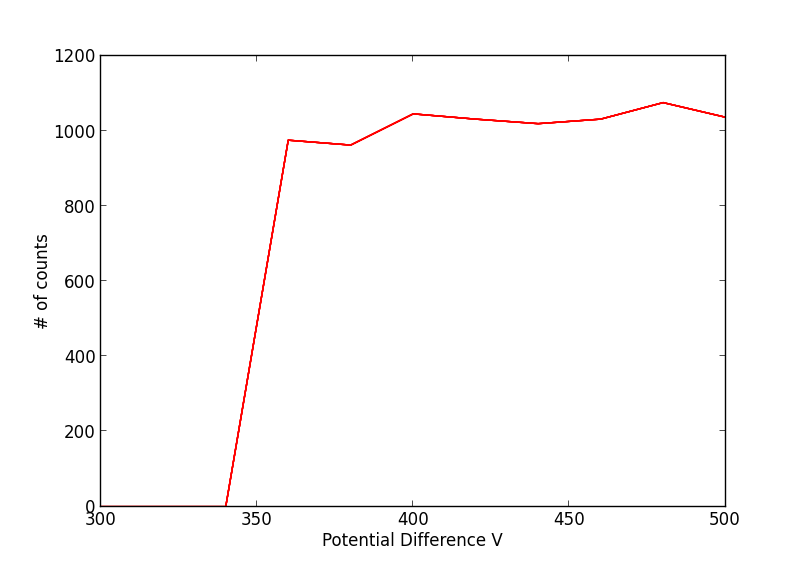
\includegraphics[width=3.5in]{potential}
\caption{The determation graph of the threshold potential}
\end{figure}

After finding the potential value, there are two steps in this experiment.In first place, there also two steps in here.
We took 100 data for each from Greiger Counter for 10 seconds near and far, and 1 second near and far at position the sensor of radioactive decay. Thus, we have 4 data set and calculated ${\chi}^{2}$, mean and standard deviation of each set by using Appendix of the course book and Python programming language.

\begin{figure}[htbp]
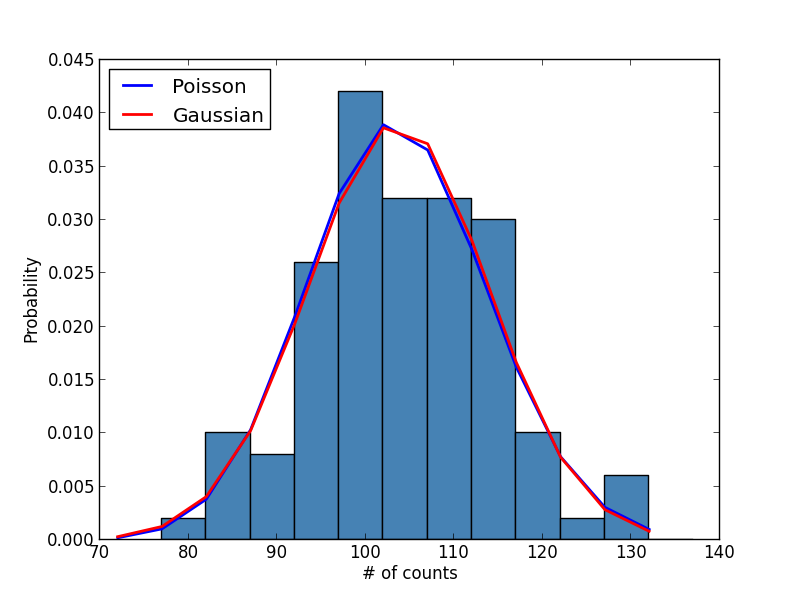
\includegraphics[width=3.5in]{tc}
\caption{10 seconds from closer bin size=5}
\end{figure}

\begin{figure}[htbp]
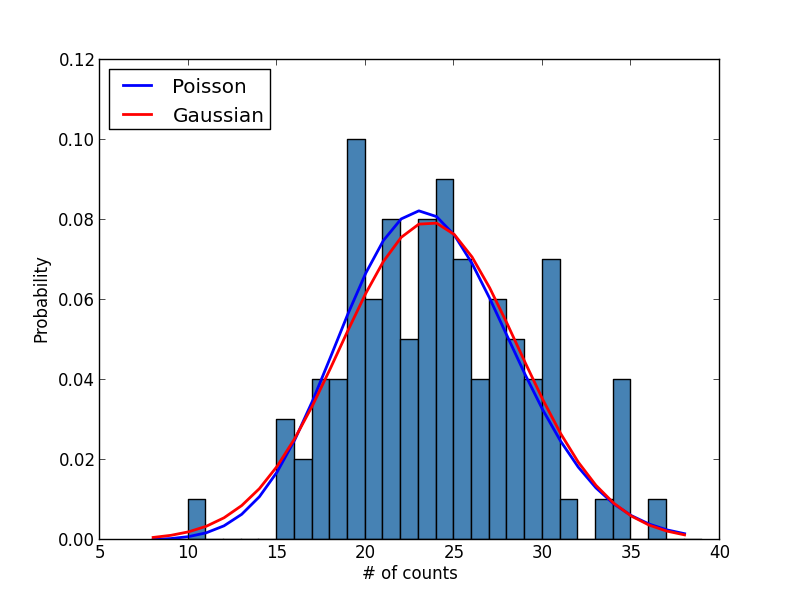
\includegraphics[width=3.5in]{tf}
\caption{10 seconds from further bin size=1}
\end{figure}

\begin{figure}[htbp]
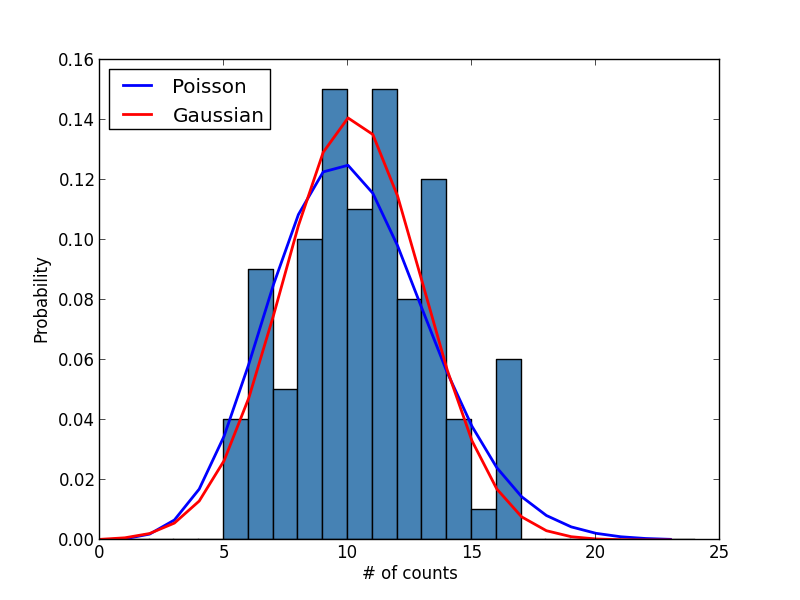
\includegraphics[width=3.5in]{oc}
\caption{1 second from closer bin size=1}
\end{figure}

\begin{figure}[htbp]
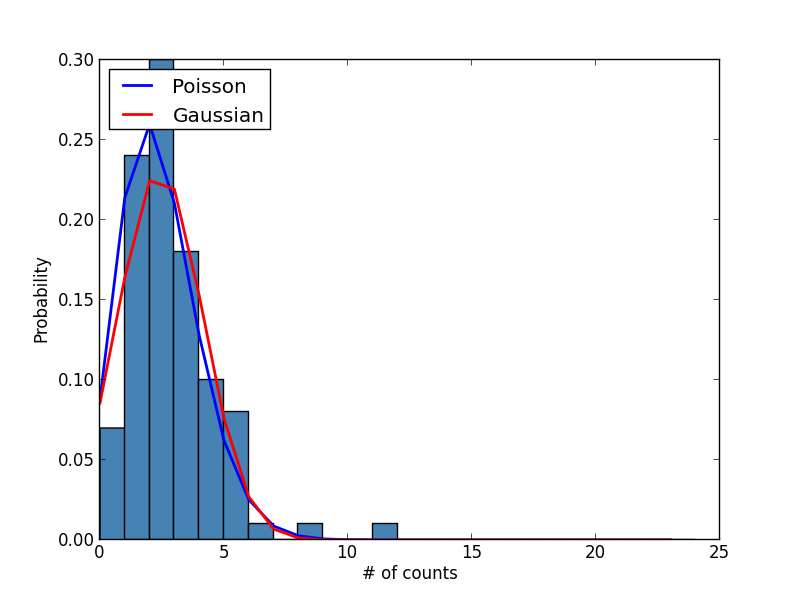
\includegraphics[width=3.5in]{of}
\caption{1 second from further bin size=1}
\end{figure}



\begin{center}
\begin{table}[htbp]
\begin{tabular}{|l|c|c|r|}
\hline
{\small number of counts} & {\small Mean ($\mu$)} & {\small Standard Deviation ($\sigma$)}  \\
\hline
10 Sec. Close 	&  103.68  	& 10.18  \\
10 Sec. Far 	&  23.58   	& 5.01  \\
1  Sec. Close 	&  10.18  	& 2.82  \\
1  Sec. Far	 	&   2.43 	& 1.72  \\
\hline
\end{tabular}
\caption{\label{tab:linfitresults} Mean and Standard Deviation for 4 data sets.}
\end{table}
\end{center}

By using ${\chi}^{2}=\sum{\frac{{({y}_{i}-f(x))}^{2}}{{\sigma}_{i}^2}}$ calculation, we found $\chi^2$ and $\frac{\chi^2}{dof}$ where $dof$ (degree of freedom) is data-1 for Poisson and data-2 for Gaussian.

\begin{center}
\begin{table}[htbp]
\begin{tabular}{|l|c|c|r|}
\hline
{\small number of counts} & {\small $\chi^2$ for Gaussian} & {\small $\chi^2/dof$ for Gaussian }  \\
\hline
10 Sec. Close 	&  0.0281  	& 0.0025  \\
10 Sec. Far 	&  0.331   	& 0.011  \\
1  Sec. Close 	&  0.253  	& 0.011  \\
1  Sec. Far	 	&  103.37 	& 4.698  \\
\hline
\end{tabular}
\caption{\label{tab:linfitresults} $\chi^2$ for Gaussian}
\end{table}
\end{center}

\begin{center}
\begin{table}[htbp]
\begin{tabular}{|l|c|c|r|}
\hline
{\small number of counts} & {\small $\chi^2$ for Poisson} & {\small $\chi^2/dof$ for Poisson}  \\
\hline
10 Sec. Close 	&  0.0281  	& 0.00234  \\
10 Sec. Far 	&  0.391   	& 0.0130  \\
1  Sec. Close 	&  0.214  	& 0.0093  \\
1  Sec. Far	 	&  2.646 	& 0.115  \\
\hline
\end{tabular}
\caption{\label{tab:linfitresults} $\chi^2$ for Poisson}
\end{table}
\end{center}

In second part, we have chart recorder and it draws events and time as $1mm$=$1\ sec.$ By binning our data for n=0 and n=1, we have two figures below:

\begin{figure}[htbp]
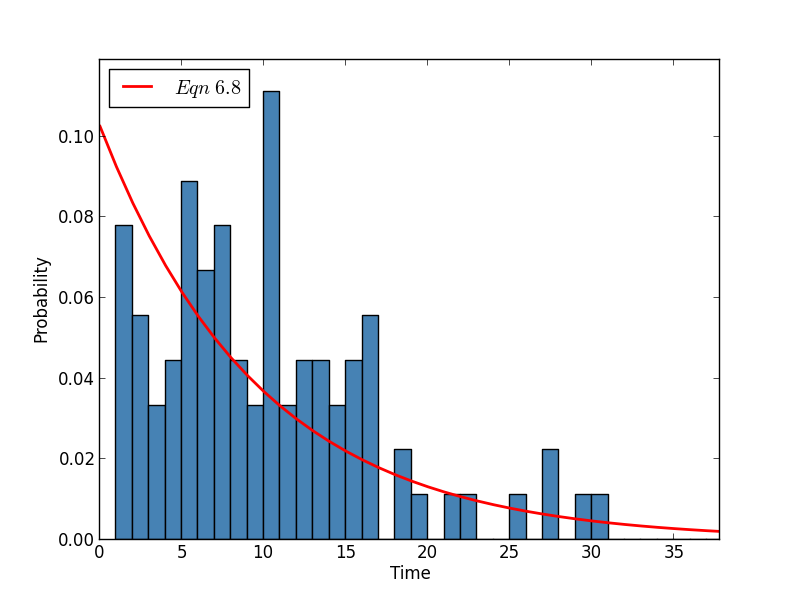
\includegraphics[width=3.5in]{n0}
\caption{n=0 Graph}
\end{figure}

\begin{figure}[htbp]
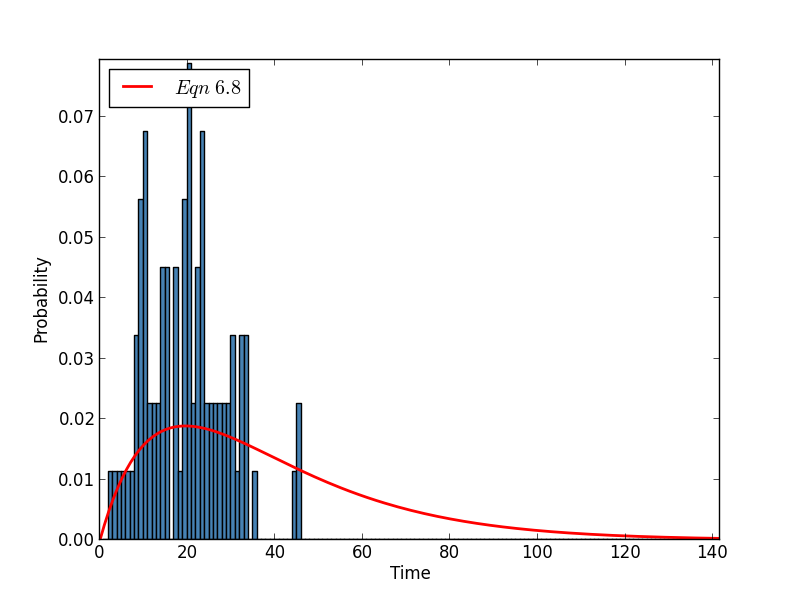
\includegraphics[width=3.5in]{n1}
\caption{n=1 Graph}
\end{figure}

where Equation 6.8 is 

\begin{center}
$P_q(n+1,t)=\frac{{(\alpha{t})}^{n}{e}^{-\alpha{t}}\alpha}{n!}$
\end{center} and $\alpha=\frac{total\ number\ of\ events}{total\ time}$.

Again $\chi^2$ calculations give:

\begin{center}
\begin{table}[htbp]
\begin{tabular}{|l|c|c|r|}
\hline
{\small $n$} & {\small Mean ($\mu$)} & {\small Standard Deviation ($\sigma$)} & {\small $\alpha$} \\
\hline
0 	&  9.744  	& 6.642  & 0.102\\
1  	&  19.505   & 9.347  &  0.051\\

\hline
\end{tabular}
\caption{\label{tab:linfitresults} Mean and Standard Deviation for 4 data sets.}
\end{table}
\end{center}

\begin{center}
\begin{table}[htbp]
\begin{tabular}{|l|c|c|r|}
\hline
{\small $n$} & {\small $\chi^2$ for Eqn 6.8} & {\small $\chi^2/dof$ for Eqn 6.8}  \\
\hline
0	&  0.600  	& 0.0006  \\
1 	&  0.741   	& 0.0007  \\

\hline
\end{tabular}
\caption{\label{tab:linfitresults} $\chi^2$ for Eqn. 6.8}
\end{table}
\end{center}




\section{Conclusions}

We have seen two examples of Poisson processes , and
have analyzed the effectiveness of the Poisson distribution as a model for these processes. For the radioactive decay, we measured the distribution of emission
events for various expected values. We found the Poisson
distribution to be a good fit for the data. However, Table I and II shows that in bigger $\mu$ values,$\chi^2$  are smaller. \\

In second part,ee have found the Poisson distribution to be an accurate description for discrete events occurring on a continuous scale.


\section{References}
\begin{itemize}
\item E. Gulmez, ”Advanced Physics Experiment”, Istanbul, Bogazici University Publication, 1999
\item http://web.mit.edu/8.13/www/experiments.shtml
\end{itemize}

\bibliography{photoelectric}




%%%%%%%%%%%%%%%%%%%%%%%%%%%%%%%%%%%%%%%%%%%%%%%%%%%%%%%%%%%%%%%%%%%%%%%%%%%%%
\begin{acknowledgments} I would like to thank my partner Kadir Simsek for his help to the experiment, and also to the teaching assistant Kazim Camlibel for his guidance during the experiment.
\end{acknowledgments}

%%%%%%%%%%%%%%%%%%%%%%%%%%%%%%%%%%%%%%%%%%%%%%%%%%%%%%%%%%%%%%%%%%%%%%%%%%%%%

\end{document}
